\documentclass[border={0.1cm 0.1cm 0.1cm 0.1cm}]{standalone}  %E,S,W,N

\usepackage{amssymb}
\usepackage{amsmath}
\usepackage{tikz}

\begin{document}
	
	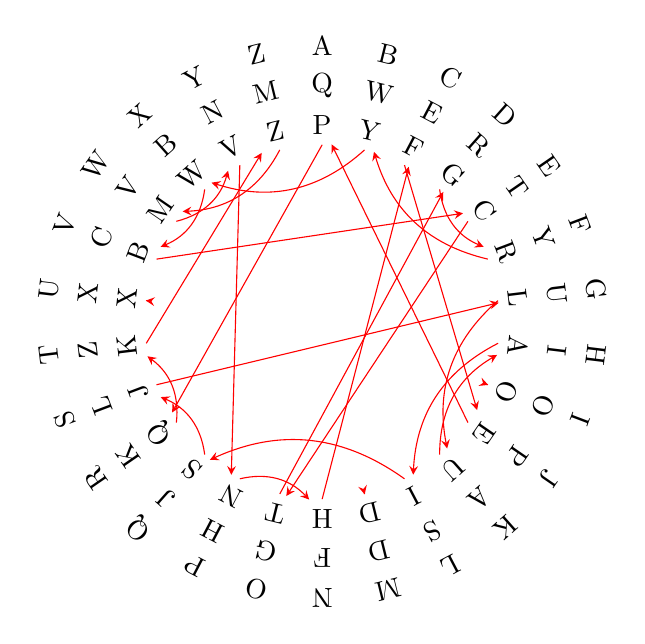
\begin{tikzpicture}[->,>=stealth]
	\foreach \i/\j/\k [count=\c from 0] in {A/Q/P,B/W/Y,C/E/F,D/R/G,E/T/C,F/Y/R,G/U/L,H/I/A,I/O/O,J/P/E, K/A/U,L/S/I,M/D/D,N/F/H,O/G/T,P/H/N,Q/J/S,R/K/Q,S/L/J,T/Z/K,U/X/X,V/C/B,W/V/M,X/B/W,Y/N/V,Z/M/Z}{
	\node[rotate={-13.846*\c}] at ({3.5*cos(90-13.846*\c)},{3.5*sin(90-13.846*\c)}) {\i};
	\node[rotate={-13.846*\c}] at ({3*cos(90-13.846*\c)},{3*sin(90-13.846*\c)}) {\j};
	\node[rotate={-13.846*\c}] (D\k) at ({2.5*cos(90-13.846*\c)},{2.5*sin(90-13.846*\c)}) {\k};
	}
	
	\draw[red] ({2.25*cos(90-13.846*0)},{2.25*sin(90-13.846*0)})--(DQ); %Q
	\draw[red] ({2.25*cos(90-13.846*1)},{2.25*sin(90-13.846*1)}) to[bend left] (DW); %W
	\draw[red] ({2.25*cos(90-13.846*2)},{2.25*sin(90-13.846*2)})--(DE); %E
	\draw[red] ({2.25*cos(90-13.846*3)},{2.25*sin(90-13.846*3)}) to[bend right] (DR); %R
	\draw[red] ({2.25*cos(90-13.846*4)},{2.25*sin(90-13.846*4)})--(DT); %T
	\draw[red] ({2.25*cos(90-13.846*5)},{2.25*sin(90-13.846*5)}) to[bend left] (DY); %Y
	\draw[red] ({2.25*cos(90-13.846*6)},{2.25*sin(90-13.846*6)}) to[bend right] (DU); %U
	\draw[red] ({2.25*cos(90-13.846*7)},{2.25*sin(90-13.846*7)}) to[bend right] (DI); %I
	\draw[red] ({2.25*cos(90-13.846*8)},{2.25*sin(90-13.846*8)})--(DO); %O %loop
	\draw[red] ({2.25*cos(90-13.846*9)},{2.25*sin(90-13.846*9)})--(DP); %P
	\draw[red] ({2.25*cos(90-13.846*10)},{2.25*sin(90-13.846*10)}) to[bend left] (DA); %A
	\draw[red] ({2.25*cos(90-13.846*11)},{2.25*sin(90-13.846*11)}) to[bend right] (DS); %S
	\draw[red] ({2.25*cos(90-13.846*12)},{2.25*sin(90-13.846*12)})--(DD); %D %loop
	\draw[red] ({2.25*cos(90-13.846*13)},{2.25*sin(90-13.846*13)})--(DF); %F
	\draw[red] ({2.25*cos(90-13.846*14)},{2.25*sin(90-13.846*14)})--(DG); %G
	\draw[red] ({2.25*cos(90-13.846*15)},{2.25*sin(90-13.846*15)}) to[bend left] (DH); %H
	\draw[red] ({2.25*cos(90-13.846*16)},{2.25*sin(90-13.846*16)}) to[bend right] (DJ); %J
	\draw[red] ({2.25*cos(90-13.846*17)},{2.25*sin(90-13.846*17)}) to[bend right] (DK); %K
	\draw[red] ({2.25*cos(90-13.846*18)},{2.25*sin(90-13.846*18)})--(DL); %L
	\draw[red] ({2.25*cos(90-13.846*19)},{2.25*sin(90-13.846*19})--(DZ); %Z
	\draw[red] ({2.25*cos(90-13.846*20)},{2.25*sin(90-13.846*20)})--(DX); %X %loop
	\draw[red] ({2.25*cos(90-13.846*21)},{2.25*sin(90-13.846*21)})--(DC); %C
	\draw[red] ({2.25*cos(90-13.846*22)},{2.25*sin(90-13.846*22)}) to[bend right] (DV); %V
	\draw[red] ({2.25*cos(90-13.846*23)},{2.25*sin(90-13.846*23)}) to[bend left] (DB); %B
	\draw[red] ({2.25*cos(90-13.846*24)},{2.25*sin(90-13.846*24)})--(DN); %N
	\draw[red] ({2.25*cos(90-13.846*25)},{2.25*sin(90-13.846*25)}) to[bend left] (DM); %M
	\end{tikzpicture}
	
\end{document}